In dieser Studie werden nur Anwendungen für das mobile Betriebssystem Android betrachtet. Da der Marktanteil von Android fast 90\% beträgt, ist dennoch ein Großteil der potenziellen NutzerInnen abgedeckt. Evaluiert werden die Anwendungen SoundWire (SW), TeamSpeak (TS) und WiFi Speaker (WFS).  Laut bestem Wissen der Autoren sind SW und WFS die einzigen beiden im Play Store verfügbaren Anwendungen, die die gewünschte Funktionalität bereitstellen (Stand: Januar 2017). Bei TS handelt es sich um eine VoIP-Anwendung, die aber so konfiguriert werden kann, dass sie ebenfalls über WiFi die Tonausgabe des PCs überträgt.

Eine herkömmliche Art die Latenz zu bestimmen, geht über das zusätzliche Senden des Zeitpunkts an dem die Tonwiedergabe am PC erfolgt ist. Die Differenz zwischen dem Zeitpunkt an dem die Tonwiedergabe am Smartphone stattgefunden hat und dem mitgesendeten Zeitpunkt entspricht der Latenz. Um diese Art der Messung durchzuführen, ist jedoch der Zugriff auf den Quellcode oder einer entsprechenden Schnittstelle der untersuchten Anwendung erforderlich. Da alle untersuchten Anwendungen proprietär sind, besteht nicht die Möglichkeit die Latenzmessungen derart durchzuführen.

Um dieses Problem zu umgehen, verwenden wir eine andere Art der Messung. Hierzu wird auf dem PC wiederholt ein Testton abgespielt. Aufgrund der Übertragungsanwendung wird der Ton verzögert auch auf dem Smartphone abgespielt. Währenddessen verwenden wir ein Mikrofon zur Aufzeichnung der Audioausgaben beider Geräte. In der anschließenden Analyse der Aufzeichnung, kann man anhand des Spektrogramms die Latenz bestimmen, vgl. Abb. 1. Vorteilhaft an diesem Ansatz ist, dass hier die Ende-zu-Ende-Verzögerung einschließlich aller Puffer-, Enkodier-, Dekodier- und Netzwerklatenzen gemessen wird. Werden programmatisch bestimmte Timestamps verwendet, besteht die Gefahr, dass die Erfassungsstelle der Timestamps falsch gewählt ist und somit bestimmte Latenzzeiten nicht ins Ergebnis einfließen.

\begin{figure}
	\begin{center}
		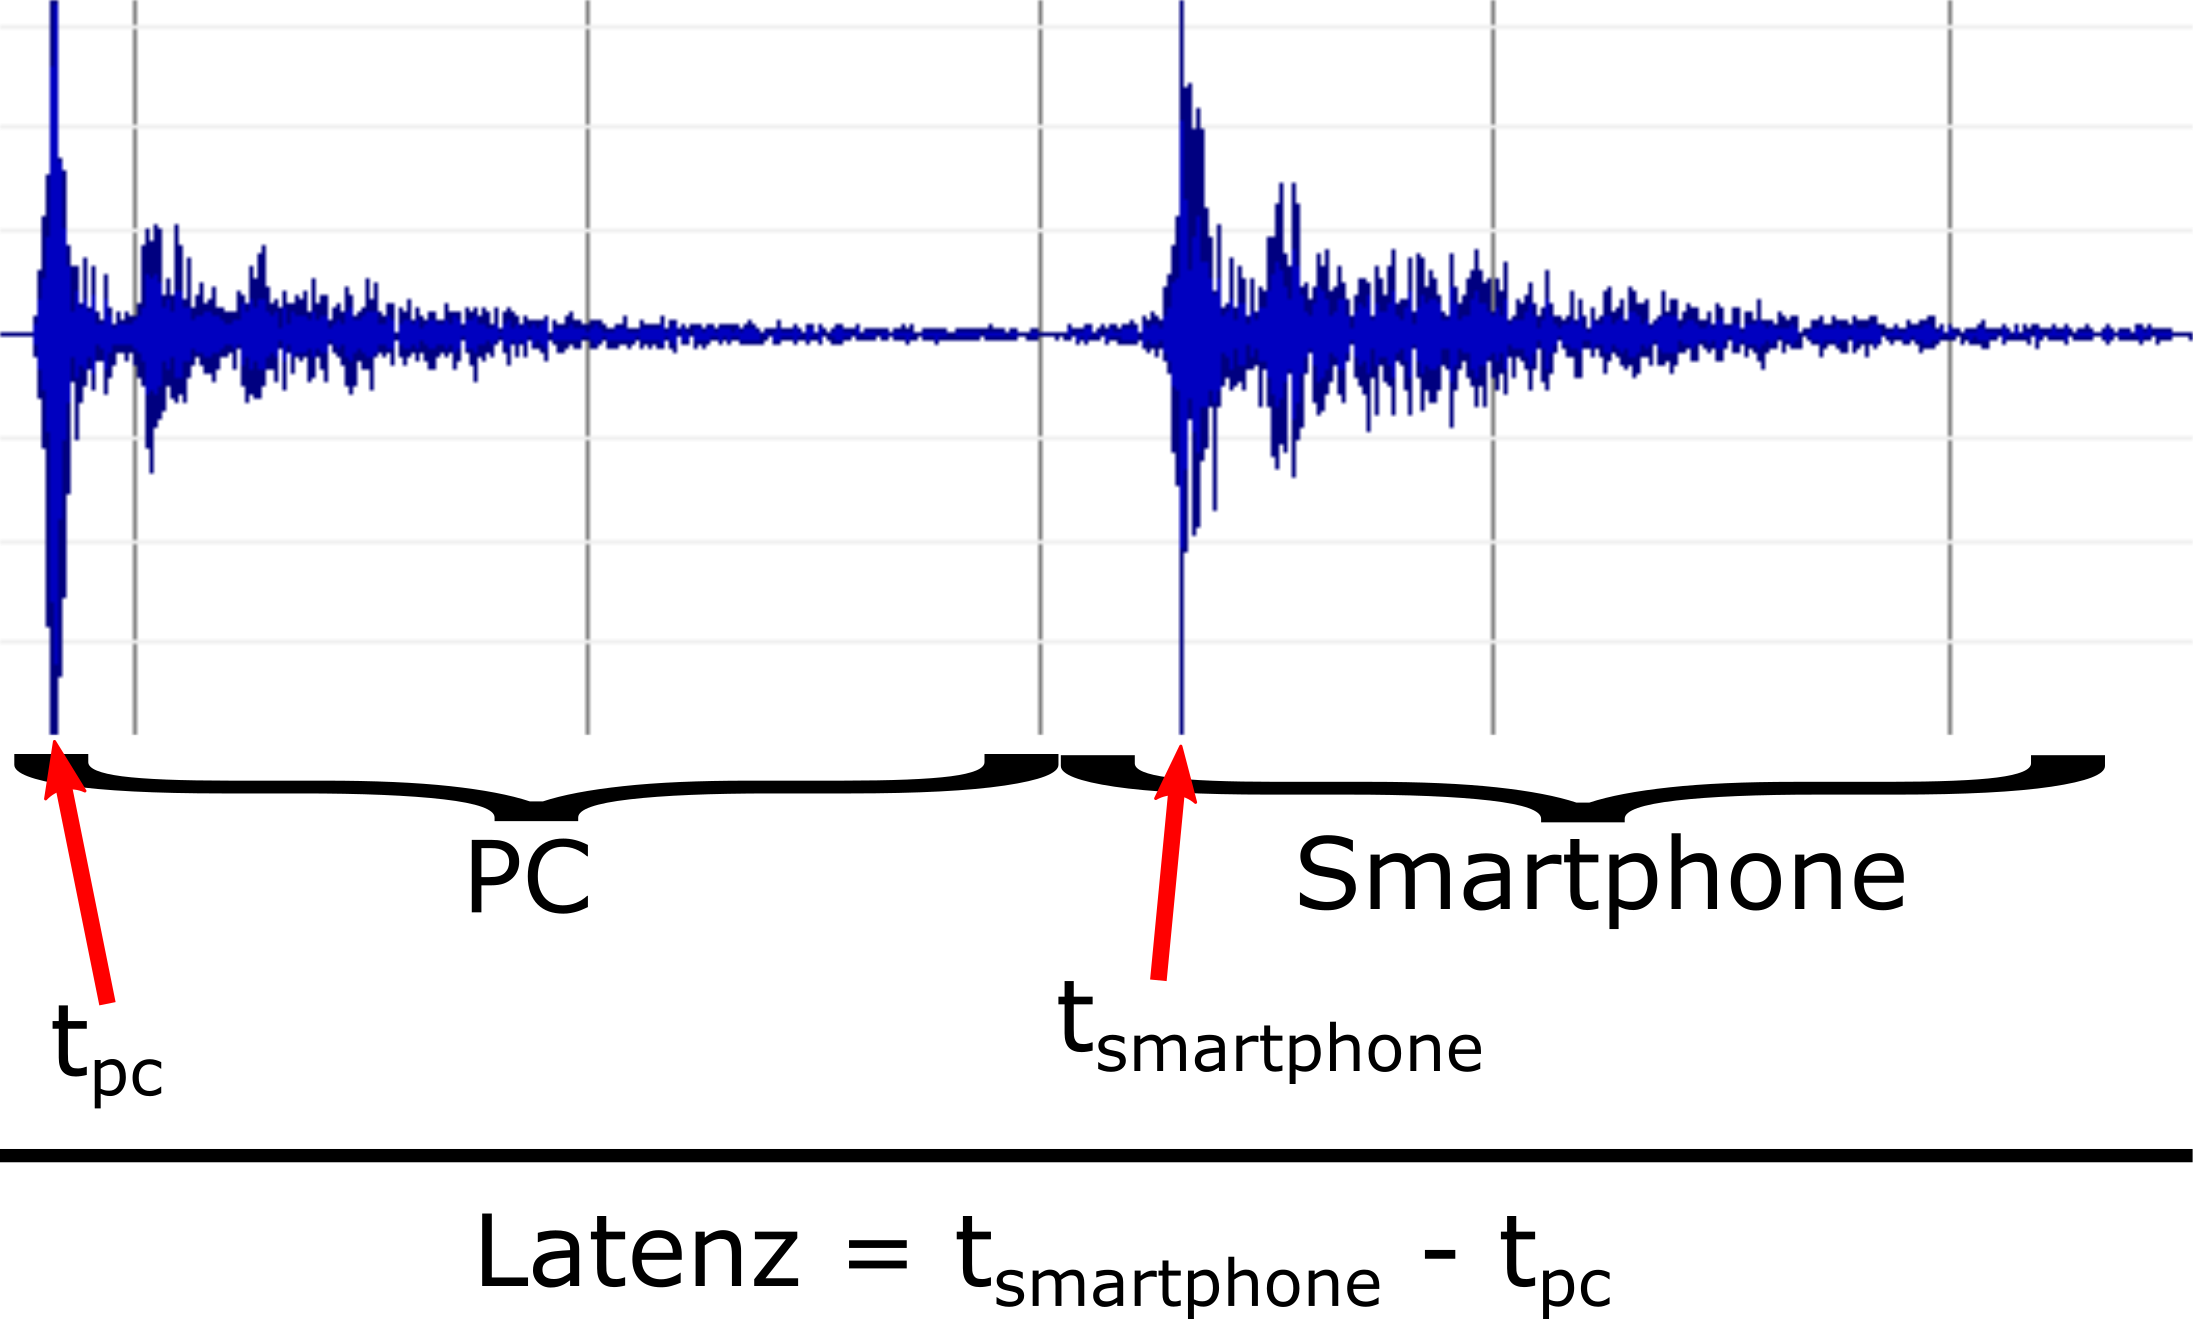
\includegraphics[width=0.5\textwidth]{img/spektrogramm.png}
		\caption{Bestimmung der Latenz anhand des Spektrogramms der Mikrofonaufnahme}
		\label{fig:spektrogramm}
	\end{center}
\end{figure}

Es wurden 30 Latenzmessungen pro Anwendung pro Smartphone aus den Leistungsklassen LOW (Samsung Galaxy S3 neo), MID (Samsung Galaxy S5) und HIGH (OnePlus 2) durchgeführt. Verwendet wurde ein PC mit Intel i7-3770k Prozessor. Die Qualität der Drahtlosübertragung kann die gemessene Latenz erheblich beeinflussen. Um den Einfluss der Übertragungsqualität einzuschränken, wurde für alle Messungen auf eine WiFi-Direct-Verbindung zurückgegriffen. Mithilfe der Anwendung Wifi Analyzer wurde zudem die Chance verringert, dass es während des Testens zu durch Interferenz verursachte Probleme kommt. Es wurde darauf geachtet, dass Audioqualität (48 kHz Stereo) und Puffergrößen bei allen Anwendungen gleich konfiguriert sind.